\documentclass[pscyr]{hedlab}
\usepackage[russian]{babel}
\usepackage{graphicx}
\graphicspath{{images/}}
\usepackage{listings}

\lstset{
  basicstyle=\footnotesize,
  inputencoding=koi8-r,
  extendedchars=True,
  language=[Sharp]C,
  numbers=left,
  numberstyle=\footnotesize,
  breakatwhitespace=\false,
  breaklines=True,
  tabsize=2,
  keepspaces=true,
}

\labname{Публикация данных в веб\\Вариант 2}
\labnum{3}
\student{Чечеткин И. А., САПР-1.1п}
\labdate{}

\begin{document}

  \makeheader

  \emph{Цель:} получение практических навыков создания базы данных СУБД
  Microsoft SQL Server Express посредством Microsoft Visual Studio и
  получения информации из таблиц базы данных в веб-приложении.
  
  \emph{Задание:}
  \begin{itemize}
    \itemsep -5pt
    \item создайте базу данных со структурой таблиц, указанной для
      соответствующего варианта;
    \item заполните таблицы не менее чем на 15 записей;
    \item создайте веб-сайт с веб-формами: для каждой таблицы создайте
      отдельную веб-форму, на которой отобразите содержимое таблицы.

  \end{itemize}
  
  Реализовать механизм передачи информации между страницами с использованием
  переменной сессии.

  \emph{Выполнение лабораторной работы:}
  В качестве исходных данных выступает структура базы данных, приведенная на
  рисунке~\ref{pic:1},
  \begin{figure}[h!]
    \vspace{-1em}\center
    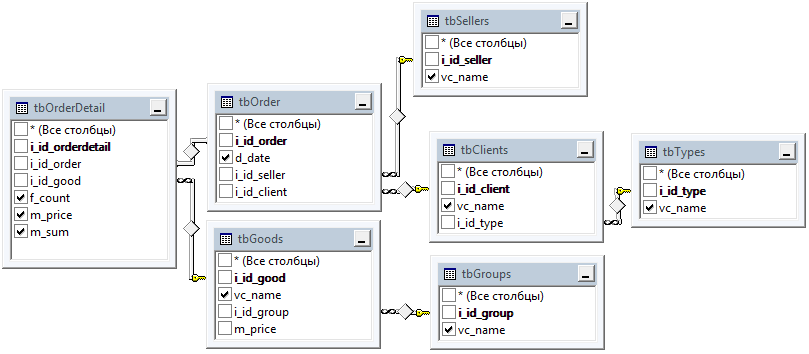
\includegraphics[width=.95\textwidth]{structure}
    \caption{Структура базы данных}
    \label{pic:1}
  \end{figure}
  
  где таблицы имеют следующую структуру:
  \begin{table}[h!]
    \caption{таблица типов клиентов tbTypes}
    \vspace{-1em}\center
    \begin{tabular}{|C{.06}|*{2}{C{.15}|}C{.3}|} \hline
      № п/п & Наименование поля & Тип & Примечание \\ \hline
      1 & i\_id\_type & Int & Primary key;
        Identity = Yes; Indentity seed = 1; Indentity~Increment~=~1 \\ \hline
      2 & vc\_name & Varchar(50) & \\ \hline
    \end{tabular}
  \end{table}
  
  \begin{table}[h!]
    \caption{таблица клиентов tbClients}
    \vspace{-1em}\center
    \begin{tabular}{|C{.06}|*{2}{C{.15}|}C{.3}|} \hline
      № п/п & Наименование поля & Тип & Примечание \\ \hline
      1 & i\_id\_client & Int & Primary key;
        Identity = Yes; Indentity seed = 1; Indentity~Increment~=~1 \\ \hline
      2 & vc\_name & Varchar(50) & Not Null;
        Default value = 'Неизвестный'\\ \hline
      3 & i\_id\_type & Int & Внешний ключ,
        ссылка на таблицу~tbTypes \\ \hline
    \end{tabular}
  \end{table}
  
  \begin{table}[h!]
    \caption{таблица продавцов tbSellers}
    \vspace{-1em}\center
    \begin{tabular}{|C{.06}|*{2}{C{.15}|}C{.3}|} \hline
      № п/п & Наименование поля & Тип & Примечание \\ \hline
      1 & i\_id\_seller & Int & Primary key;
        Identity = Yes; Indentity seed = 1; Indentity~Increment~=~1 \\ \hline
      2 & vc\_name & Varchar(50) & Not Null;
        Default value = 'Иванов~Иван~Иванович'\\ \hline
    \end{tabular}
  \end{table}
  
  \begin{table}[h!]
    \caption{таблица групп товаров tbGroups}
    \vspace{-1em}\center
    \begin{tabular}{|C{.06}|*{2}{C{.15}|}C{.3}|} \hline
      № п/п & Наименование поля & Тип & Примечание \\ \hline
      1 & i\_id\_group & Int & Primary key;
        Identity = Yes; Indentity seed = 1; Indentity~Increment~=~1 \\ \hline
      2 & vc\_name & Varchar(50) & \\ \hline
    \end{tabular}
  \end{table}
  
  \begin{table}[h!]
    \caption{таблица товаров tbGoods}
    \vspace{-1em}\center
    \begin{tabular}{|C{.06}|*{2}{C{.15}|}C{.3}|} \hline
      № п/п & Наименование поля & Тип & Примечание \\ \hline
      1 & i\_id\_good & Int & Primary key;
        Identity = Yes; Indentity seed = 1; Indentity~Increment~=~1 \\ \hline
      2 & vc\_name & Varchar(50) & Not Null;
        Default value = 'Товар' \\ \hline
      3 & i\_id\_group & Int & Внешний ключ,
        ссылка на таблицу~tbGroups \\ \hline
      4 & m\_price & Money & Not Null;
        Defaul value = 0.00 \\ \hline
    \end{tabular}
  \end{table}
  
  \clearpage
  
  \begin{table}[h!]
    \caption{таблица шапки документов <<заказы>> tbOrder}
    \vspace{-1em}\center
    \begin{tabular}{|C{.06}|*{2}{C{.15}|}C{.3}|} \hline
      № п/п & Наименование поля & Тип & Примечание \\ \hline
      1 & i\_id\_order & Int & Primary key;
        Identity = Yes; Indentity seed = 1; Indentity~Increment~=~1 \\ \hline
      2 & d\_date & Datetime & Not Null \\ \hline
      3 & i\_id\_seller & Int & Внешний ключ,
        ссылка на таблицу~tbSellers \\ \hline
      4 & i\_id\_client & Int & Внешний ключ,
        ссылка на таблицу~tbClients \\ \hline
    \end{tabular}
  \end{table}
  
  \begin{table}[h!]
    \caption{таблица табличной части документа <<заказы>> tbOrderDetail}
    \vspace{-1em}\center
    \begin{tabular}{|C{.06}|*{2}{C{.15}|}C{.3}|} \hline
      № п/п & Наименование поля & Тип & Примечание \\ \hline
      1 & i\_id\_orderdetail & Int & Primary key;
        Identity = Yes; Indentity seed = 1; Indentity~Increment~=~1 \\ \hline
      2 & i\_id\_order & Int & Внешний ключ,
        ссылка на таблицу~tbOrder \\ \hline
      3 & i\_id\_good & Int & Внешний ключ,
        ссылка на таблицу~tbGoods \\ \hline
      4 & f\_count & Float & Количество \\ \hline
      5 & m\_price & Money & Цена \\ \hline
      6 & m\_sum & Money & Сумма \\ \hline
    \end{tabular}
  \end{table}
  
  В Visual Studio:
  \begin{figure}[h!]
    \center
    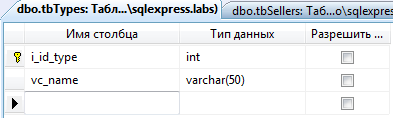
\includegraphics[width=.47\textwidth]{types_tab} \hspace{1em}
    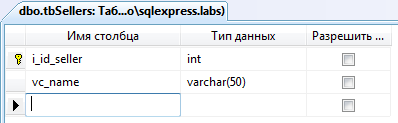
\includegraphics[width=.47\textwidth]{sellers_tab} \\[.5em]
    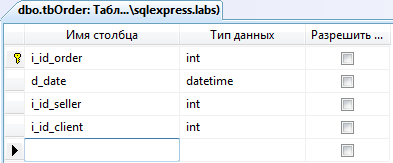
\includegraphics[width=.47\textwidth]{order_tab} \hspace{1em}
    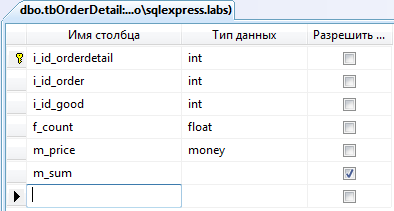
\includegraphics[width=.47\textwidth]{orderdetail_tab}
  \end{figure}
  
  \newpage
  
  \begin{figure}[h!]
    \center
    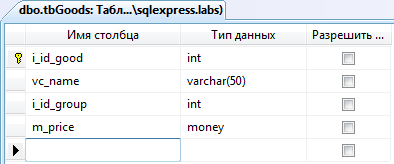
\includegraphics[width=.47\textwidth]{goods_tab} \hspace{1em}
    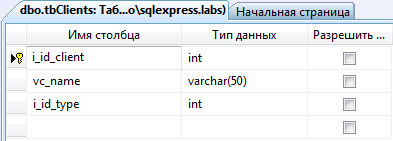
\includegraphics[width=.47\textwidth]{clients_tab} \\[.5em]
    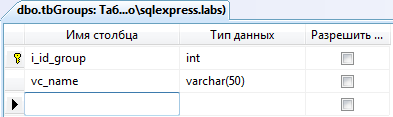
\includegraphics[width=.47\textwidth]{groups_tab}
  \end{figure}
  
  Скриншоты страниц:
  \begin{figure}[h!]
    \center
    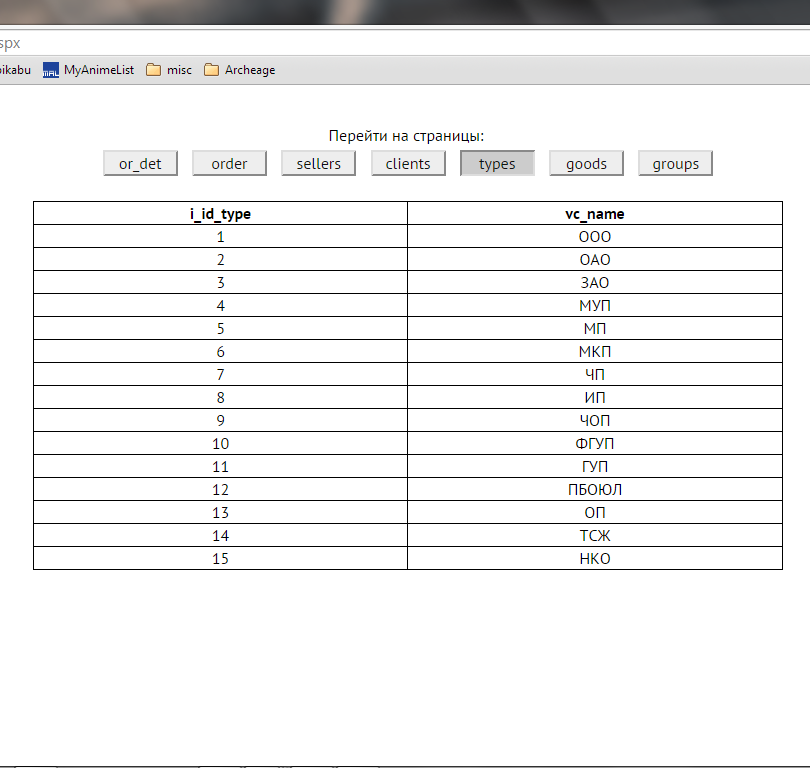
\includegraphics[width=.47\textwidth]{types} \hspace{1em}
    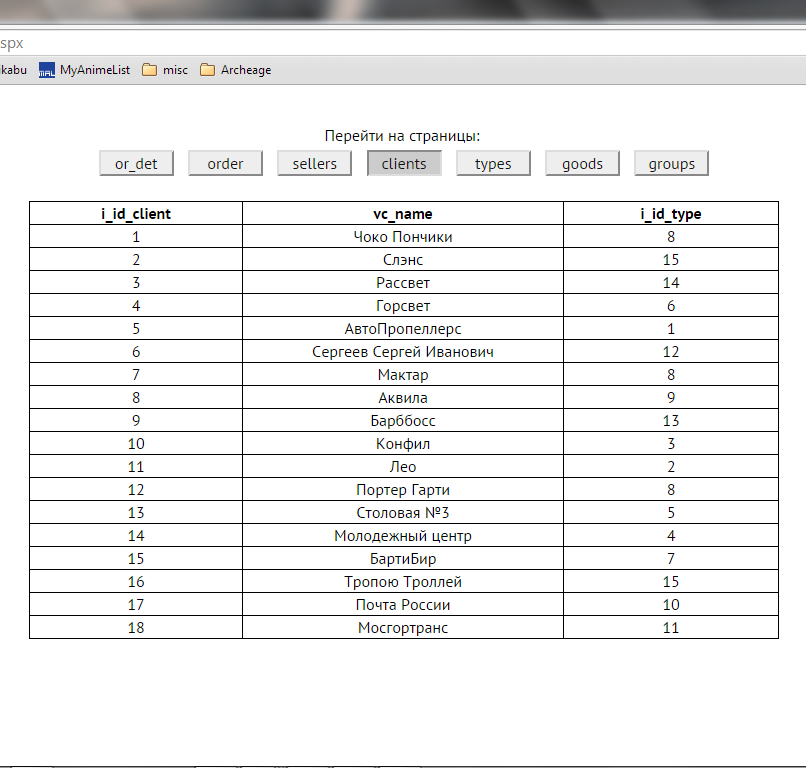
\includegraphics[width=.47\textwidth]{clients} \\
    \parbox{.47\textwidth}{\caption{Types}} \hspace{1em}
    \parbox{.47\textwidth}{\caption{Clients}} \\
    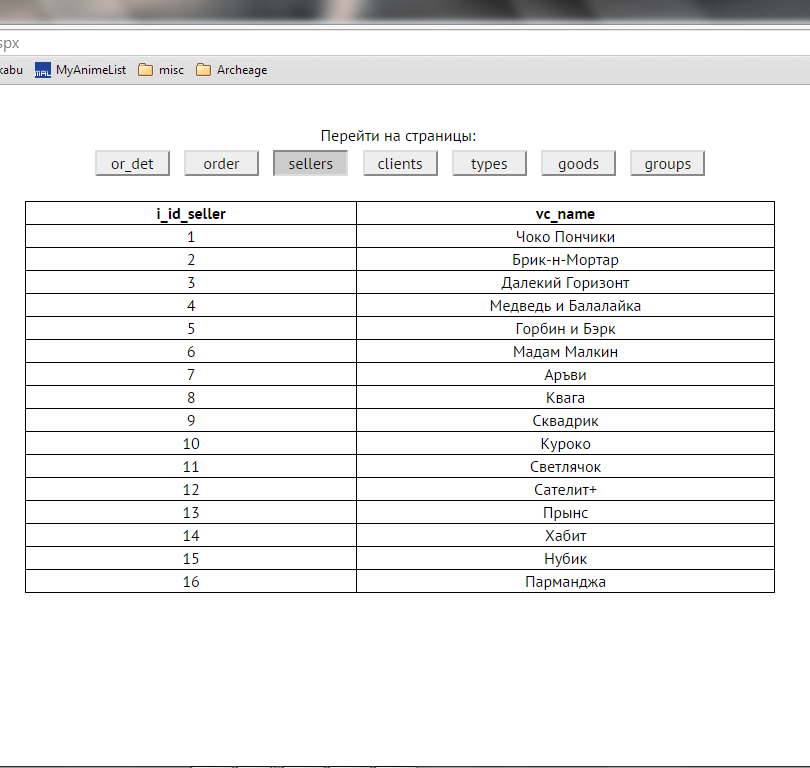
\includegraphics[width=.47\textwidth]{sellers} \hspace{1em}
    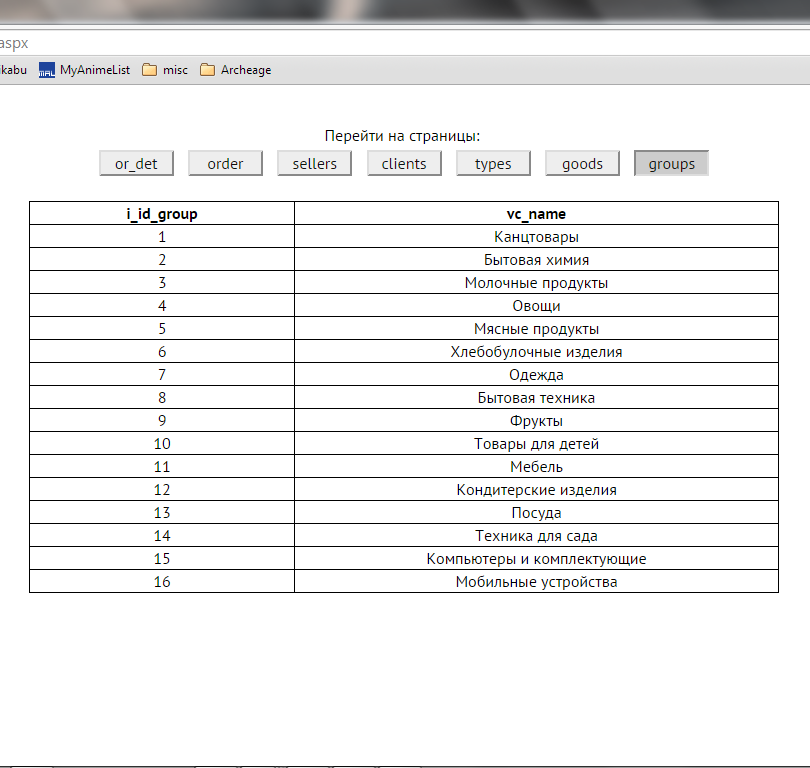
\includegraphics[width=.47\textwidth]{groups} \\
    \parbox{.47\textwidth}{\caption{Sellers}} \hspace{1em}
    \parbox{.47\textwidth}{\caption{Groups}}
  \end{figure}
  
  \newpage
  
  \begin{figure}[h!]
    \center
    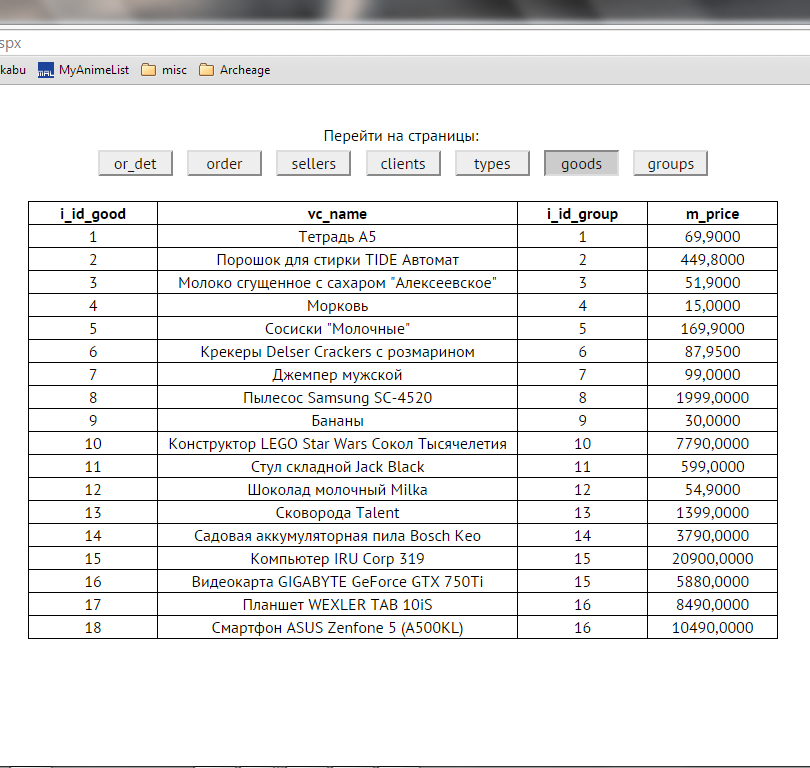
\includegraphics[width=.47\textwidth]{goods} \hspace{1em}
    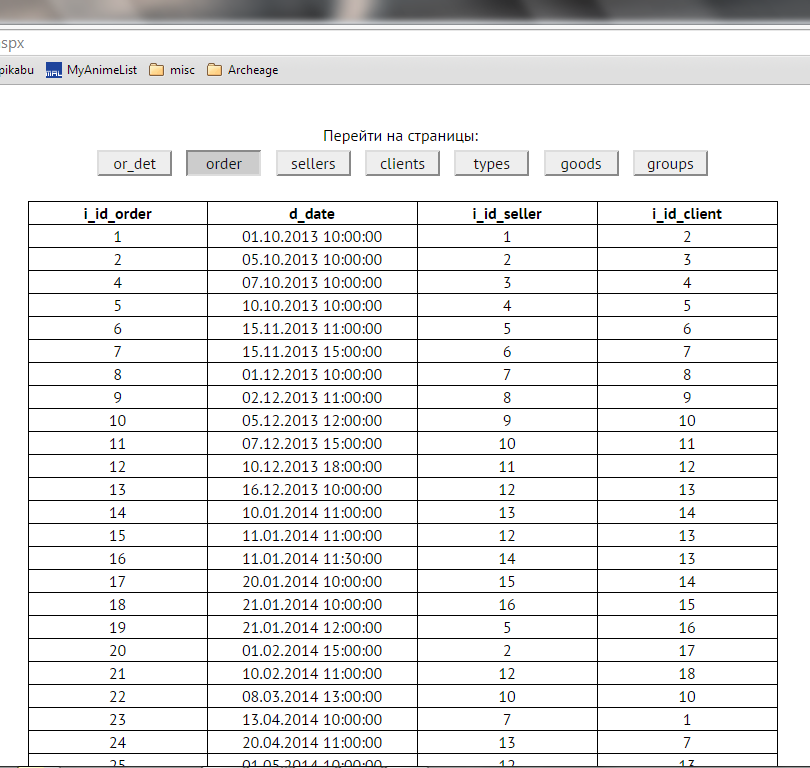
\includegraphics[width=.47\textwidth]{order} \\
    \parbox{.47\textwidth}{\caption{Goods}} \hspace{1em}
    \parbox{.47\textwidth}{\caption{Order}} \\
    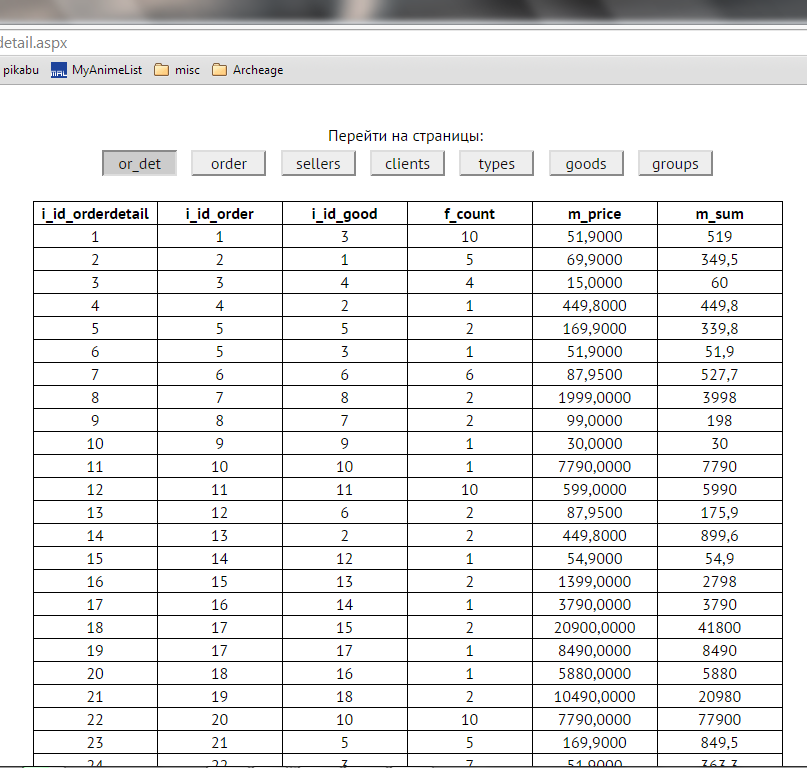
\includegraphics[width=.6\textwidth]{orderdetail}
    \caption{OrderDetail}
  \end{figure}
  
  Пример кода страницы и классов кода страницы (страница OrderDetail).\\
  \textbf{orderdetail.aspx}:
  \lstinputlisting[language=HTML]{code/orderdetail.aspx}
  
  \vspace{2em}
  \textbf{orderdetail.cs}:
  \lstinputlisting{code/orderdetail.cs}
  
  \emph{Вывод:} в результате проделанной работы
  \vspace{-.5em}  
  \begin{enumerate}
    \itemsep -5pt
    \item создал проект веб-сайта;
    \item создал базу данных, таблицы базы данных согласно заданию и
      наполнил таблицы информацией;
    \item создал объект SQLDataSource и настроил его на получение информации
      из связанных таблиц;
    \item реализовал метод получения данных из таблиц и отображения их на
      странице веб-сайта.
  \end{enumerate}

\end{document}